\documentclass[DIN, pagenumber=false, fontsize=11pt, parskip=half]{scrartcl}

\usepackage{amsmath}
\usepackage{amsfonts}
\usepackage{amssymb}
\usepackage{enumitem}
\usepackage[utf8]{inputenc} 
\usepackage[ngerman]{babel} 
\usepackage[T1]{fontenc} 
\usepackage{pgfplots}
\usepackage{xcolor}
\usepackage{listings}
\usepackage{float}
\usepackage{graphicx}
\usepackage{svg}
\usepackage{booktabs}
\usepackage{gensymb}
\usepackage{dcolumn}


\definecolor{mygreen}{RGB}{28,172,0} % color values Red, Green, Blue
\definecolor{mylilas}{RGB}{170,55,241}

\newcommand{\norm}[1]{\left\lVert#1\right\rVert}

\lstset{language=Matlab,%
    %basicstyle=\color{red},
    breaklines=true,%
    morekeywords={matlab2tikz},
    keywordstyle=\color{blue},%
    morekeywords=[2]{1}, keywordstyle=[2]{\color{black}},
    identifierstyle=\color{black},%
    stringstyle=\color{mylilas},
    commentstyle=\color{mygreen},%
    showstringspaces=false,%without this there will be a symbol in the places where there is a space
    numbers=left,%
    numberstyle={\tiny \color{black}},% size of the numbers
    numbersep=9pt, % this defines how far the numbers are from the text
    emph=[1]{for,end,break},emphstyle=[1]\color{red}, %some words to emphasise
    %emph=[2]{word1,word2}, emphstyle=[2]{style},    
}

\DeclareUnicodeCharacter{00B0}{\degree}


\title{Computer Vision I}
\author{Tim Luchterhand, Paul Nykiel (Group 17)}

\begin{document}
    \maketitle
    \section{Moravec Operator}
    \lstinputlisting{sh04ex01.m}
    \begin{figure}[H]
        \centering
        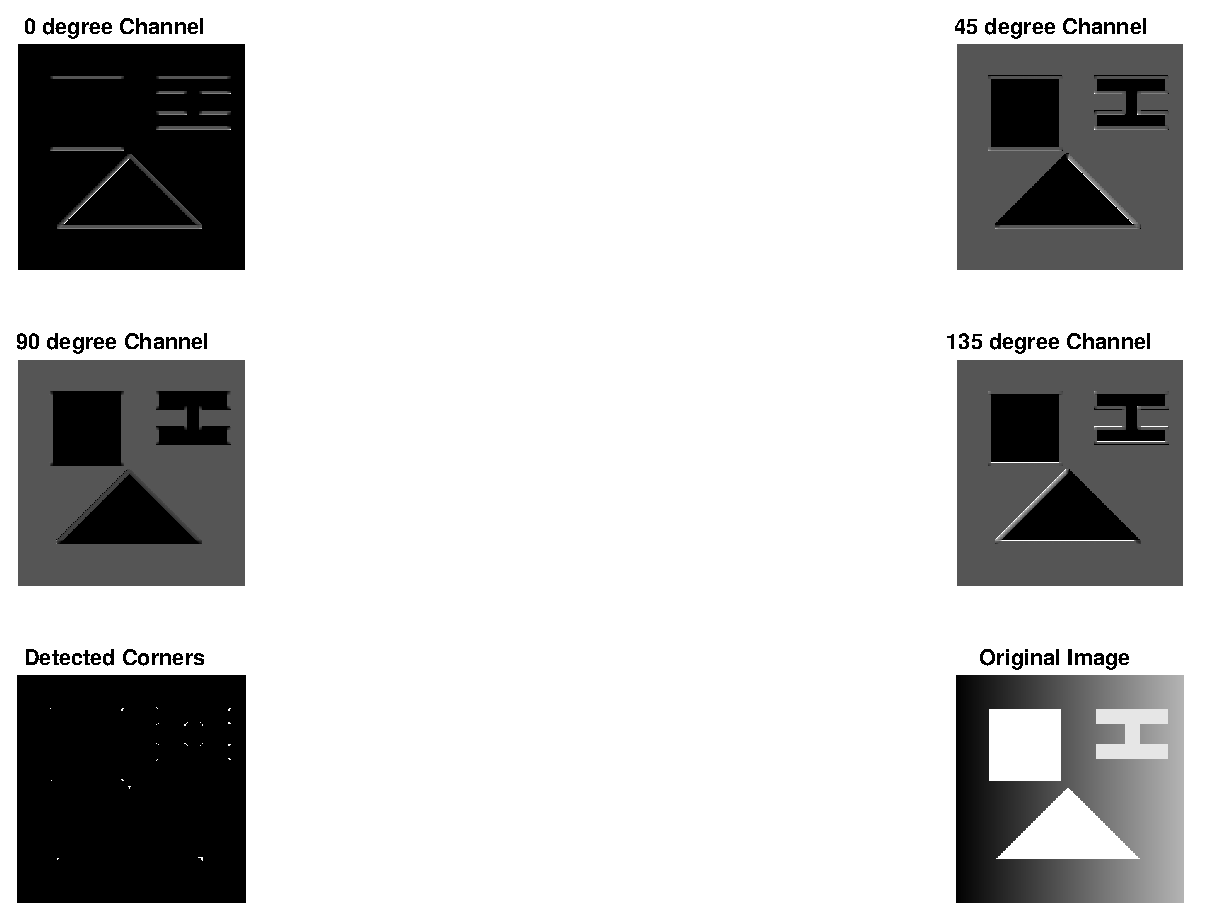
\includegraphics[width=\textwidth]{sh04ex01.eps}
    \end{figure}
    Uncorrelated noise has a high frequency and is therefor strongly amplified by the derivation. As a result there are a lot more false positives in the image.
    To achieve better results one could use a low-pass-filter to surpress high frequencys (in this case the noise). This can be done by convolving the image with
    a gaussian kernel.

    \section{Structure Tensor}
    \lstinputlisting{sh04ex02.m}
    \begin{figure}[H]
        \centering
        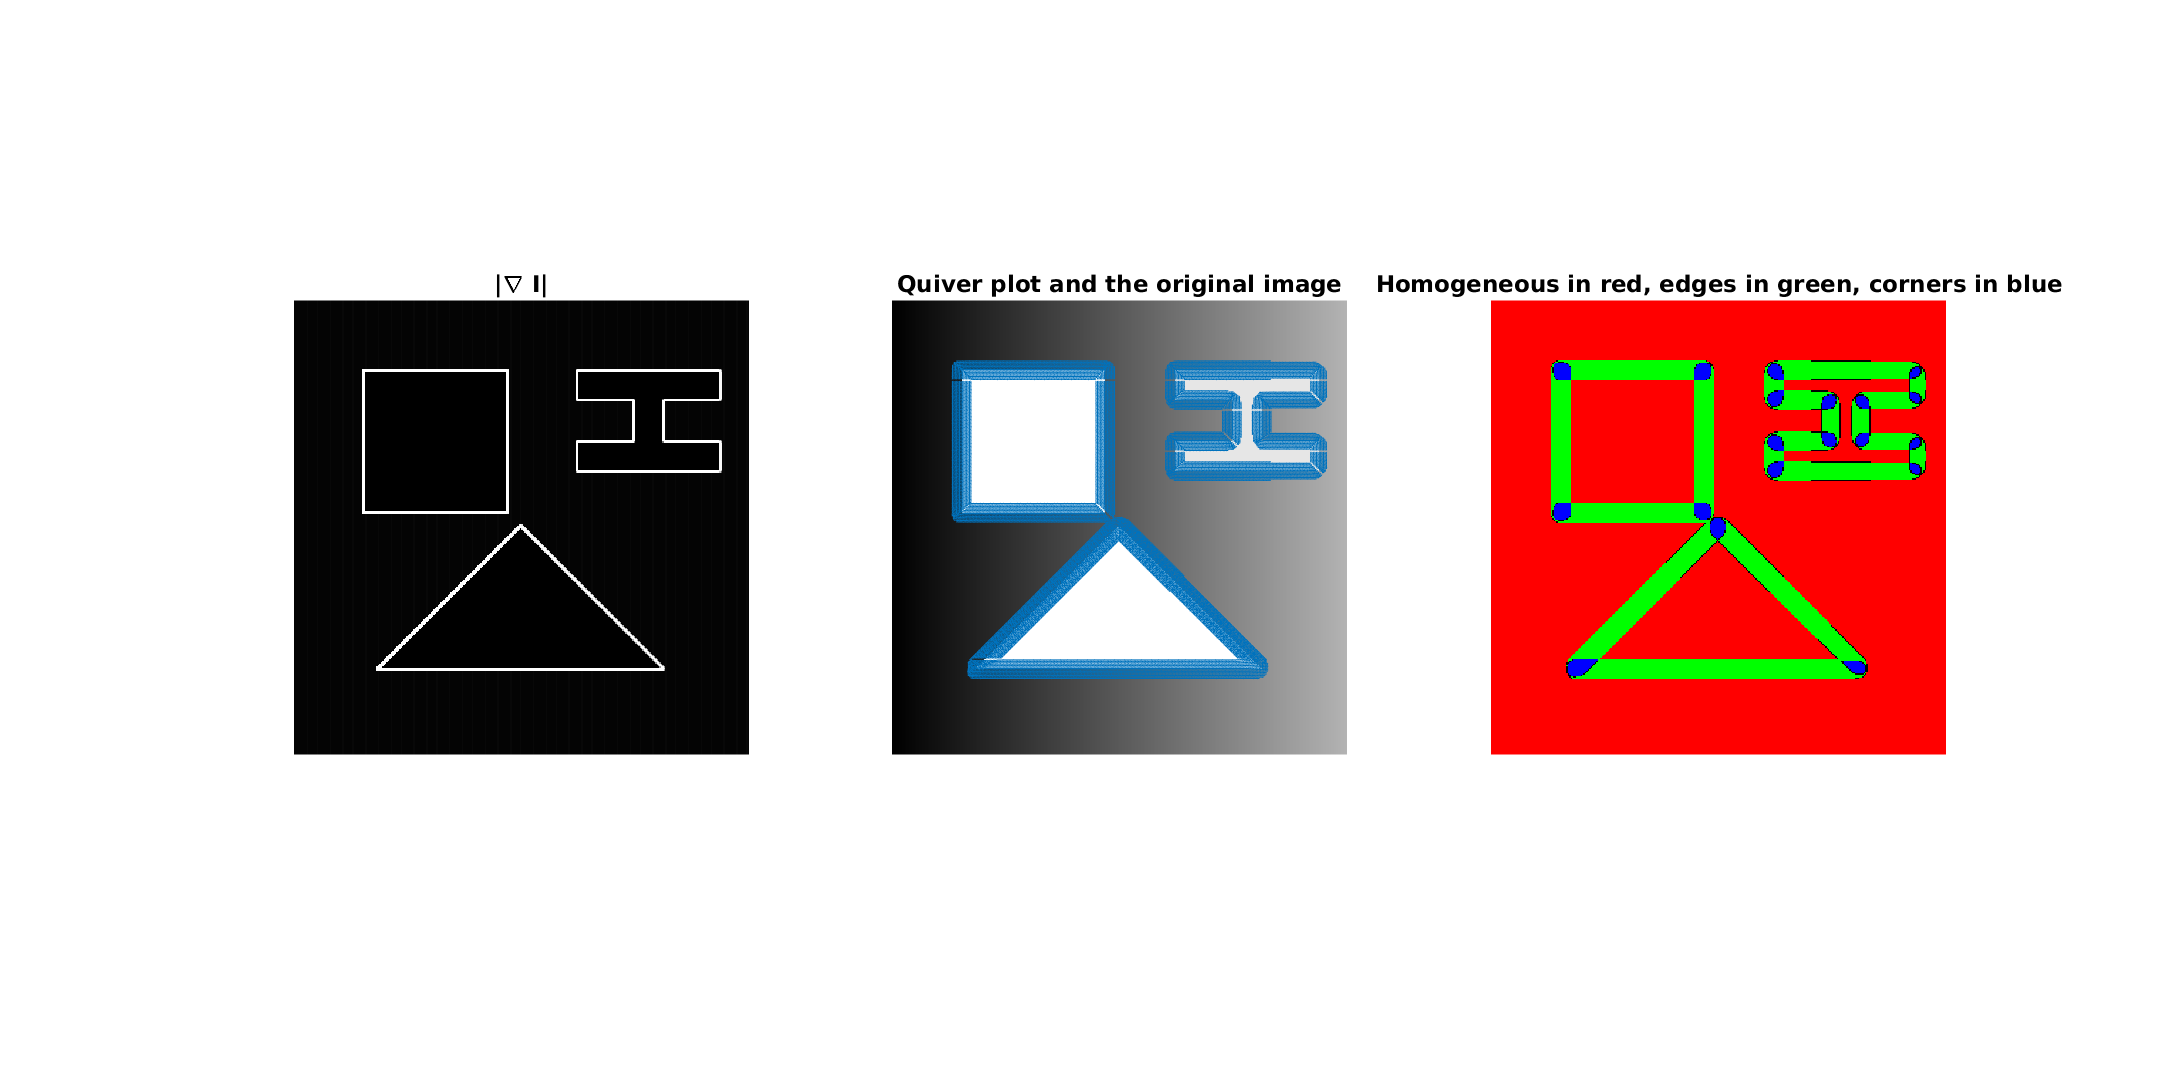
\includegraphics[width=\textwidth]{sh04ex02.eps}
    \end{figure}
\end{document}
